% This is "sig-alternate.tex" V2.0 May 2012
% This file should be compiled with V2.5 of "sig-alternate.cls" May 2012
%
% This example file demonstrates the use of the 'sig-alternate.cls'
% V2.5 LaTeX2e document class file. It is for those submitting
% articles to ACM Conference Proceedings WHO DO NOT WISH TO
% STRICTLY ADHERE TO THE SIGS (PUBS-BOARD-ENDORSED) STYLE.
% The 'sig-alternate.cls' file will produce a similar-looking,
% albeit, 'tighter' paper resulting in, invariably, fewer pages.
%
% ----------------------------------------------------------------------------------------------------------------
% This .tex file (and associated .cls V2.5) produces:
%       1) The Permission Statement
%       2) The Conference (location) Info information
%       3) The Copyright Line with ACM data
%       4) NO page numbers
%
% as against the acm_proc_article-sp.cls file which
% DOES NOT produce 1) thru' 3) above.
%
% Using 'sig-alternate.cls' you have control, however, from within
% the source .tex file, over both the CopyrightYear
% (defaulted to 200X) and the ACM Copyright Data
% (defaulted to X-XXXXX-XX-X/XX/XX).
% e.g.
% \CopyrightYear{2007} will cause 2007 to appear in the copyright line.
% \crdata{0-12345-67-8/90/12} will cause 0-12345-67-8/90/12 to appear in the copyright line.
%
% ---------------------------------------------------------------------------------------------------------------
% This .tex source is an example which *does* use
% the .bib file (from which the .bbl file % is produced).
% REMEMBER HOWEVER: After having produced the .bbl file,
% and prior to final submission, you *NEED* to 'insert'
% your .bbl file into your source .tex file so as to provide
% ONE 'self-contained' source file.
%
% ================= IF YOU HAVE QUESTIONS =======================
% Questions regarding the SIGS styles, SIGS policies and
% procedures, Conferences etc. should be sent to
% Adrienne Griscti (griscti@acm.org)
%
% Technical questions _only_ to
% Gerald Murray (murray@hq.acm.org)
% ===============================================================
%
% For tracking purposes - this is V2.0 - May 2012

\documentclass{sig-alternate}
\begin{document}
\conferenceinfo{GECCO'15,} {July 11-15, 2015, Madrid, Spain.}
\CopyrightYear{2015}
\crdata{TBA}
\clubpenalty=10000
\widowpenalty = 10000
%
% --- Author Metadata here ---
%\conferenceinfo{WOODSTOCK}{'97 El Paso, Texas USA}
%\CopyrightYear{2007} % Allows default copyright year (20XX) to be over-ridden - IF NEED BE.
%\crdata{0-12345-67-8/90/01}  % Allows default copyright data (0-89791-88-6/97/05) to be over-ridden - IF NEED BE.
% --- End of Author Metadata ---

\title{Harnessing changing environments for avoiding premature
convergence}%\titlenote{(Produces the permission block, and
%copyright information). For use with
%SIG-ALTERNATE.CLS. Supported by ACM.}}
\subtitle{[Evolution Strategies and Evolutionary Programming Track]
%\titlenote{A full version of this paper is available as
%\textit{Author's Guide to Preparing ACM SIG Proceedings Using
%\LaTeX$2_\epsilon$\ and BibTeX} at
%\texttt{www.acm.org/eaddress.htm}}}
}
%
% You need the command \numberofauthors to handle the 'placement
% and alignment' of the authors beneath the title.
%
% For aesthetic reasons, we recommend 'three authors at a time'
% i.e. three 'name/affiliation blocks' be placed beneath the title.
%
% NOTE: You are NOT restricted in how many 'rows' of
% "name/affiliations" may appear. We just ask that you restrict
% the number of 'columns' to three.
%
% Because of the available 'opening page real-estate'
% we ask you to refrain from putting more than six authors
% (two rows with three columns) beneath the article title.
% More than six makes the first-page appear very cluttered indeed.
%
% Use the \alignauthor commands to handle the names
% and affiliations for an 'aesthetic maximum' of six authors.
% Add names, affiliations, addresses for
% the seventh etc. author(s) as the argument for the
% \additionalauthors command.
% These 'additional authors' will be output/set for you
% without further effort on your part as the last section in
% the body of your article BEFORE References or any Appendices.

\numberofauthors{4} %  in this sample file, there are a *total*
% of EIGHT authors. SIX appear on the 'first-page' (for formatting
% reasons) and the remaining two appear in the \additionalauthors section.
%
\author{
% You can go ahead and credit any number of authors here,
% e.g. one 'row of three' or two rows (consisting of one row of three
% and a second row of one, two or three).
%
% The command \alignauthor (no curly braces needed) should
% precede each author name, affiliation/snail-mail address and
% e-mail address. Additionally, tag each line of
% affiliation/address with \affaddr, and tag the
% e-mail address with \email.
%
% 1st. author
\alignauthor
Emily Dolson\\%\titlenote{This author supervised the coding, carried out the experiments, analyzed the data, and wrote the paper}\\
       \affaddr{BEACON Center for the Study of Evolution in Action}\\
       \affaddr{Michigan State University}\\
       \affaddr{East Lansing, U.S.A.}\\
       \email{dolsonem@msu.edu}
% 2nd. author
\alignauthor Joshua Nahum\\%\titlenote{This author assisted in all aspects of this project}\\
       \affaddr{BEACON Center for the Study of Evolution in Action}\\
       \affaddr{Michigan State University}\\
       \affaddr{East Lansing, U.S.A.}\\
%       \email{webmaster@marysville-ohio.com}
%3rd. author
\alignauthor
Riley Annis\\%\titlenote{With assistance from the first two authors, this author wrote the majority of the code for this project.}\\
       \affaddr{BEACON Center for the Study of Evolution in Action}\\
       \affaddr{Michigan State University}\\
       \affaddr{East Lansing, U.S.A.}\\
\and  % use '\and' if you need 'another row' of author names
% 4th. author
\alignauthor Charles Ofria\\%\titlenote{This author supervised all aspects of this project.}\\
 	   \affaddr{BEACON Center for the Study of Evolution in Action}\\
       \affaddr{Michigan State University}\\
       \affaddr{East Lansing, U.S.A.}\\%       
       %\email{lleipuner@researchlabs.org}
% 5th. author
%\alignauthor Sean Fogarty\\
%       \affaddr{NASA Ames Research Center}\\
%       \affaddr{Moffett Field}\\
%       \affaddr{California 94035}\\
%       \email{fogartys@amesres.org}
% 6th. author
%\alignauthor Charles Palmer\\
%       \affaddr{Palmer Research Laboratories}\\
%       \affaddr{8600 Datapoint Drive}\\
%       \affaddr{San Antonio, Texas 78229}\\
%       \email{cpalmer@prl.com}
}
% There's nothing stopping you putting the seventh, eighth, etc.
% author on the opening page (as the 'third row') but we ask,
% for aesthetic reasons that you place these 'additional authors'
% in the \additional authors block, viz.
%\additionalauthors{Additional authors: John Smith (The Th{\o}rv{\"a}ld Group,
%email: {\texttt{jsmith@affiliation.org}}) and Julius P.~Kumquat
%(The Kumquat Consortium, email: {\texttt{jpkumquat@consortium.net}}).}
\date{9 December 2014}
% Just remember to make sure that the TOTAL number of authors
% is the number that will appear on the first page PLUS the
% number that will appear in the \additionalauthors section.

\maketitle
\begin{abstract}
Despite the biological theory suggesting that changing environments may promote improved adaptation across environments, the concept of using changing environments to improve results in evolutionary computation has gotten little attention. Preliminary results in Avida and NK-Landscapes suggest that temporarily moving a population to an environment with only a slight correlation to the original environment can promote higher fitness when the population is moved back to the original environment. Here, we seek to determine whether or not these results generalize to real-valued vector problems. By super-imposing a random landscape of peaks and valleys onto mathematical optimization benchmark functions, we create alternative landscapes to place populations in. Results suggest that, while this technique can be slightly harmful to overall fitness for very easy problems (such as the sphere function), it usually has no clear effect on fitness. However, preliminary results suggest that, for substantially harder problems (e.g. versions of these standard benchmarks with large numbers of parameters) than those used here, switching to a different environment can substantially increase the variance in average fitnesses attained by a given population. This results in the potential for both substantially better and substantially worse results than if the population were continuously left in the same environment. Further research is needed to better understand the parameter ranges in which these different behaviors are exhibited.
\end{abstract}

% A category with the (minimum) three required fields
%\category{H.4}{Information Systems Applications}{Miscellaneous}
%A category including the fourth, optional field follows...
%\category{D.2.8}{Software Engineering}{Metrics}[complexity measures, performance measures]

%\terms{Theory}

\keywords{Changing environments, real-valued optimization, evolutionary computation}

\section{Introduction}
In nature, the environment in which populations are evolving is constantly changing. This can take the form of large scale shifts, such as global climate change, or subtle adjustments, such as the influx of soil nutrients that occurs when a tree falls in a forest and begins decomposing. This change can present hardships or benefits to any given species in the short term. In the long term, changing environments are often attributed to the evolution of generally useful attributes, such as intelligence\cite{parter_facilitated_2008}. In evolutionary computation, however, changing environments are typically viewed as a nuisance to be avoided. There has been a fair amount of research on how to use evolutionary computation to solve problems that are, in reality, constantly changing, but few have explored the potential benefits of exposure to general alternate environments.

A number of techniques that have previously been found to be useful involve changing the environment in which evolution is occurring. Fitness sharing\cite{goldberg_genetic_1987} and novelty search\cite{lehman_abandoning_2011}, for instance, depress the fitness landscape in the vicinity of common or previously discovered solutions. Many "stepping stone" approaches, in which the population is given progressively more challenging problems to solve (for example: \cite{harper_spatial_2012}), are also fundamentally examples of changing environments. All of these techniques, however, involve using environments that differ from the environment of interest in very specific ways. The theory that changing environments promote the development of generally useful skills, on the other hand, would suggest that exposure to a wide variety of different environments should be useful.

The one context in evolutionary computation in which changing environments have been used as an intentional driver of adaptation is in the context of encouraging genetic modularity. Indeed, they have had a great deal of success in this domain\cite{ovaska_periodical_2009}\cite{intelligent_systems_group_department_of_computer_science_university_of_bath_bath_ba1_7ay_u.k._evolving_2014}.  Recently, Kashtan et al found that this has the convenient side effect of increasing the speed with which the optimal solution is found\cite{kashtan_varying_2007}. Intriguingly, Kashtan et al observed this result even in a condition that was not explicitly designed to be modular.

Preliminary data support the theory that exposure to alternative environments should be generally useful to evolutionary computation, even in the absence of a specific need for modularity. A study using the Avida Digital Evolution Platform found that placing a population in the environment of interest for the first third of evolutionary time, moving it to a different environment for the middle third, and then moving it back to the original environment for the final third resulted in the population attaining higher average fitness in the original environment \cite{nahum_improved_????}. However, it could be argued that, since environments in Avida are defined by the set of boolean logic functions that are rewarded, this is effectively a "stepping stone" scenario; the environments are likely to make use of the same building blocks, because any logic function is likely to be useful in computing additional logic functions. On some level, of course, shared building blocks are the reason that a change in environments is likely to be useful. But environments involving shared building blocks are trivially created in Avida to a much greater extent than in most more applied evolutionary computation systems. As such, it is relevant to ask whether these results generalize to systems other than Avida.

Thus far, these results have only been replicated in the NK-Landscape model. In this study, populations were again evolved in a single environment for the first and last third of evolution and placed in a different environment for the middle third. The amount of correlation between the two environments was varied. Populations that spent time in an environment with an intermediate correlation to the original environment attained higher fitness in the original environment than populations that were either kept in the same fitness landscape for all of evolutionary time or transferred to an environment that was strongly negatively correlated with the original environment\cite{nahum_unpublished_????}.

The fact that these results hold for NK-Landscapes is promising, and raises the question of how far they can be generalized. Are changing environments useful for solving actual problems? Here we explore the efficacy of this technique for evolutionary algorithms attempting to solve real-valued vector optimization problems. Real-valued vector optimization problems were selected for their clear practical usefulness and the ease of visualizing changes to their fitness landscapes.

\section{Methods}
Genotypes were represented as vectors of real-valued numbers. Populations were evolved in one environment, represented by a standard real-valued optimization benchmark function, for the first and last third of evolutionary time. For the middle third of evolution, the populations were placed in an alternate environment.

\subsection{Creating alternative environments}
There are a wide variety of ways in which it would be possible to create an alternative fitness landscape. Adjusting the parameter values of a specific function, for instance, or combining two functions both have the potential to be useful. In order for the results of this study to be generally applicable, however, we avoid using any such problem-specific techniques here. Instead, we overlay a randomly generated fitness landscape on top of the landscape of the problem being solved. To accomplish this, a set of values along each dimension of the problem is selected to serve as "anchor" points for the random overlay landscape. For each of these values, a random number is selected. This number represents the "adjustment value" to be added to any locus in the genotype vector which has a value equal to the anchor point. By interpolating between anchor points, we can obtain adjustment values for any gene value. This results in a randomly generated set of peaks and valleys being superimposed on the original fitness landscape.

While the goal of creating alternate environments in this way is to create a technique that is easily generalizable, it is important to keep in mind that the random landscapes it creates have certain commonalities. They are generally symmetric across dimensions and non-differentiable, for instance.  There are a wide variety of alternative ways in which mostly-random fitness landscapes could theoretically be generated, which may or may not be worthy of further investigation. 

Another important issue to keep in mind when it comes to alternate environments is how to quantify them. The metric used here is correlation between the alternative environment and the original environment. This is computed by selecting 5000 random points across the problem space and calculating the value in both environments. A least-squares regression of fitness in the alternate environment on fitness in the original environment is performed. The correlation is the r value of this regression. This metric has the advantage of being highly general and straightforward, but the disadvantage of not capturing much information about the way in which the environments differ. For instance, systematic differences in the magnitude of values in one environment vs. the other are completely invisible to the correlation metric.

\begin{figure*}
\centering
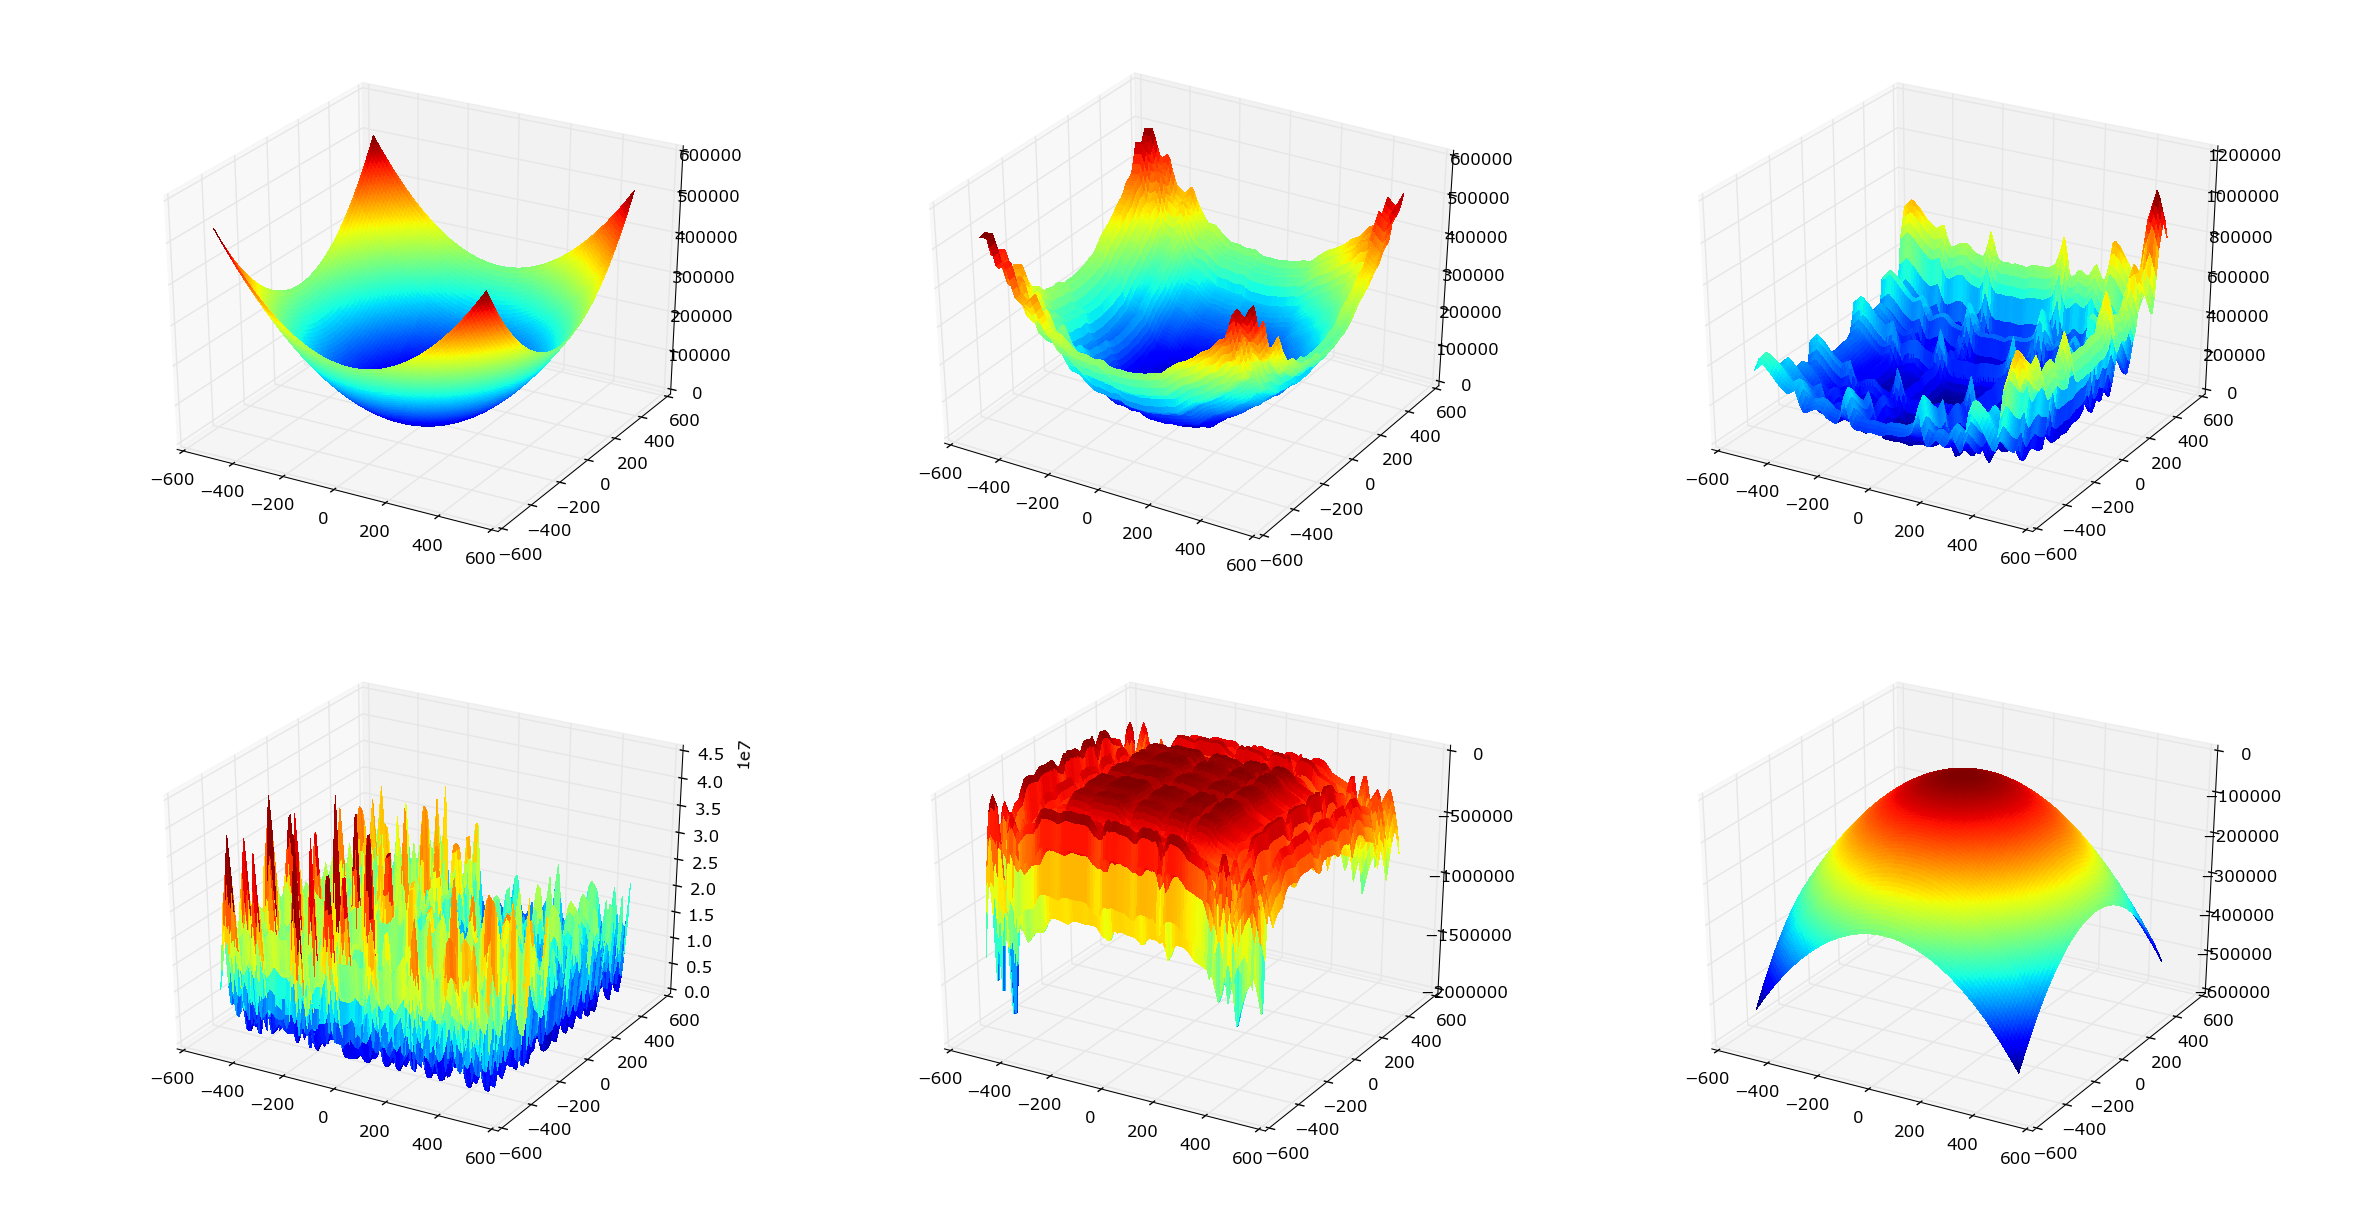
\psfig{file=/home/emily/repos/ChangingEnvironmentGA/alternate_sphere_functions.ps, scale=.32}
\caption{Examples of alternate environments for the sphere function with different amounts of correlation to 
the standard problem. Correlations (left to right, top to bottom) are: 1, 0.99, 0.77, 0.23, -0.66, and -1}
\end{figure*}

Alternative environments with correlations to the original environment ranging from -1 to 1 were used. Since a correlation of 1 exactly reproduces the original environment, this was used as a control. Results from the NK-Landscape experiments suggest that a correlation of -1 should be harmful to adaption to the original environment, but it is included here for completeness. For examples of what alternate environments with different correlations look like, see Figure 1.

\subsection{The Genetic Algorithm}
To minimize the potential for unexpected interactions between changing environments and the underlying algorithm doing the evolution, we used the most simplistic evolutionary algorithm that was still capable of solving the simplest of our problems (the sphere function). In the tradition of previous work done on real-valued vector problems, this algorithm allowed mutation but no crossover. Mutation rate was set at .2, meaning that each locus in the vector had a 20\% chance of experiencing a mutation. Mutations added a random number drawn from a normal distribution with a mean of 0 and a standard deviation of 10 to the value in question. Mutations that would push a value beyond the allowed range (specified individually for each problem) instead caused the value to wrap around to the opposite edge of this range. Tournament selection with a tournament size of 10 was used as a selection operator. Population size was kept at 500. All source code for the algorithm and analysis of results is available on the author's GitHub page: https://github.com/emilydolson/ChangingEnvironmentGA, and is written in Python 2.7 with extensive use of the NumPy, SciPy\cite{jones_scipy:_2001}, and MatPlotLib\cite{hunter_matplotlib:_2007} libraries. All functions were tested with a vector length of 20 over the course of 2500 generations.

In response to the better-than-expected performance of the minimalistic evolutionary algorithm on these problems, a set of experiments on the Schaffer F7 function were run with a vector length of 100 over the course of 5000 generations.

A diversity maintenance scheme (restricted tournament selection) was tested and found to have no effect. As such, results from it are not included in this paper.

\subsection{The Benchmark Functions}
A variety of benchmark functions were used, with the goal of understanding under what scenarios it can be useful for a population to evolve in an alternate environment over the course of evolutionary time. All function definitions were taken from the website accompanying \cite{holtschulte_should_2013}.

\subsubsection{Sphere Function}
The sphere function is a very straightforward, smooth, unimodal minimization problem.
\begin{displaymath}f(x_1 \cdots x_n) = \sum_{i=1}^n x_i^2\end{displaymath}
\begin{displaymath}-512 \leq x_i \leq 512\end{displaymath}
\begin{displaymath}\text{minimum at }f(0, \cdots, 0) = 0\end{displaymath}

\subsubsection{Rosenbrock Function}
The Rosenbrock function is also smooth and unimodal, but features a fairly large valley that it can be challenging to find the lowest point in.
\begin{displaymath}f(x_1 \cdots x_n) = \sum_{i=1}^{n-1} (100(x_i^2 - x_{i+1})^2 + (1-x_i)^2)\end{displaymath}
\begin{displaymath}-2.048 \leq x_i \leq 2.048\end{displaymath}
\begin{displaymath}\text{minimum at }f(1, 1, \cdots, 1) = 0\end{displaymath}

\subsubsection{Rana Function}
The Rana function is a complex, multimodal function. There is some disagreement in the literature as to what the minimum is, but it seems to occur somewhere in the vicinity of $x_i = -512$. 
\begin{displaymath}f(x_i \cdots x_n)=x_i sin(\sqrt{|x_{i+1}+1-x_i|})cos(\sqrt{|x_i+x_{i+1}+1|})\end{displaymath}
\begin{displaymath} + (x_{i+1}+1)cos(\sqrt{|x_{i+1}+1-x_i|})sin(\sqrt{|x_i+x_{i+1}+1|})\end{displaymath}
\begin{displaymath}-512 \leq x_i \leq 512\end{displaymath}

\subsubsection{Schaffer's F7 Function}
Schaffer's F7 function is a deceptive and multimodal function in which solutions must cross a series of high ridges to find progressively lower valleys.
\begin{displaymath}f(x_0 \cdots x_n) = [\frac{1}{n-1}\sqrt{s_i} \cdot (sin(50.0s_i^{\frac{1}{5}})+1)]^2 \end{displaymath}
where
\begin{displaymath}s_i = \sqrt{x_i^2 + x_{i+1}^2}\end{displaymath}
\begin{displaymath}-512 \leq x_i \leq 512\end{displaymath}
\begin{displaymath}\text{minimum at }f(0, \cdots, 0) = 0\end{displaymath}

\section{Results}

Changing environments typically resulted in a sudden drastic loss of fitness as measured in the original environment. Fitness as measured in the original environment then stabilized until the population was returned to it, at which point fitness generally improved rapidly once again.

For the experiments with vector lengths of 20 (see Figure 2), there was no significant difference (linear regression, p = .96) among the average or best fitnesses achieved under different conditions. The one exception to this trend was the sphere function, for which switching to an alternate environment for part of evolution had a negative impact on final fitness. As predicted, this impact was most negative for the condition in which the alternative environment was the exact inverse of the original environment. 

\begin{figure*}
\centering
\psfig{file=/media/emily/hdd/changing_environments_data/longer_run_many/runs_over_time_all_sphere_2500gen_best.ps, scale=.4}\psfig{file=/media/emily/hdd/changing_environments_data/longer_run_many/runs_over_time_all_rosenbrock_2500gen_best.ps, scale=.4}
\psfig{file=/media/emily/hdd/changing_environments_data/longer_run_many/runs_over_time_all_rana_2500gen.ps, scale=.3} \psfig{file=/media/emily/hdd/changing_environments_data/longer_run_many/runs_over_time_all_schaffer_2500gen_best.ps, scale=.4}
\caption{Theses graphs show the log of fitness (in the original environment) over the course of evolutionary time for each of the four problems. Lines are colored by the correlation between the alternate and original environments. From left to right, top to bottom, the graphs represent results from the sphere function, Rosenbrock function, Rana function, and Schaffer F7 function. Each graph contains the results of 500 runs of the algorithm, 100 of which had a correlation of 1, and 100 of which had a correlation of -1. Note that lower fitnesses are better, and as such fitness in the original environment gets dramatically worse while the population is in the alternative environment for the middle third of evolution. The exceptions to this are the runs in which the alternative environment is identical to the original environment (correlation=1).}
\end{figure*}

In the experiment with vector lengths of 100 (see Figure 3), the set of populations that spent the middle third of evolution in an environment with near-zero correlation to their original environment had substantially greater variation in average final fitnesses than did the set of populations that stayed in the same environment the whole time. As a result, a number of populations that changed environments attained better average fitnesses than any population that didn't. However, a number of populations that changed environments also attained much worse average fitnesses than any population that didn't. A linear regression of average final fitness on correlation of alternative environment suggested that spending time in an a different environment has a tiny but significant positive impact on overall fitness (slope=-0.002, intercept = 0.367, p-value = .007). It is possible that this is explained by random variation in the starting conditions; a number of populations that happened to be in the group that were put in alternative environments were performing very well before the switch.
\begin{figure}
\centering
\psfig{file=/media/emily/hdd/changing_environments_data/length_100/runs_over_time_all_schaffer_2500gen_best.ps, scale=.5} \psfig{file=/media/emily/hdd/changing_environments_data/length_100/correlation_vs_final_fitness_scatter_schaffer_avergae.ps, scale=.5}
\caption{(Top) Log of fitness (in the original environment) over the course of evolutionary time for the 100-parameter Schaffer F7 function. Lines are colored by the correlation between the alternate and original environments. (Bottom) Scatter plot showing correlation between original and alternate environments on the x axis, and log of average fitness of the population after 5000 generations on the y axis.}
\end{figure}

Changing environments incurs minimal computational overhead. Figuring out how to appropriately adjust values while evaluating fitness in the alternate environment takes O(n) time, which is the same complexity as evaluating fitness in the original environment. There is a slight additional memory overhead for the hash table storing the values associated with each anchor point.

\section{Discussion and Conclusions}
The fitness trajectories in the different conditions behaved qualitatively as expected. They initially improved rapidly before stagnating. When placed in a different environment, fitness in that environment rapidly rose at the cost of fitness in the original environment. This trend is quickly reversed when the population is moved back to the original environment. All of these results are consistent with those obtained by previous research, suggesting that the fundamental set-up of the system is sound.

For easy (i.e. smooth and unimodal) problems, it seems that changing environments may be slightly harmful to evolution. This makes sense, as no innovation is required to solve such problems; getting to new areas of the fitness landscape isn't particularly useful. For most other problems, there seems to be no clear benefit or harm in changing environments.

The 100-parameter version of the Schaffer F7 function, however, provides evidence that there are circumstances under which changing environments can make a difference. While there seem to be roughly even odds that that difference will be negative vs. positive, the potential for generating substantially better solutions may make this technique attractive under certain circumstances. It is also possible that various parameter adjustments, such as allowing more evolution to occur after the population is returned to the original environment, might help reduce the likelihood of changing environments yielding dramatically worse results. 

Ultimately, these results are inconclusive, due to the narrow portion of parameter space explored thus far. However, they have the potential to form the basis of a counterpoint to the idea that changing environments are broadly helpful across all forms of evolutionary computation.

\section{Future Work}
In order to understand the broader implications of these results a few things will be necessary. First of all, performing tests in which one copy of a starting population is moved to a different environment for part of evolutionary time and another copy of the same population is not would be very valuable in ensuring that these results are not due to chance. Second, testing larger problem sizes for the other benchmarks will be important. As a deceptive problem, the Schaffer F7 function may be uniquely positioned to be benefited by a change of environment. Third, testing more benchmark problems is also likely a good idea, as there may be specific properties of the fitness landscape that interact with the effects of changing environments. Finally, testing a wider range of parameters for creating the alternative environment, and controlling the amount of time spent in each environment will help ensure that the parameter space is well-understood.

\section{Acknowledgments}
We extend our thanks to Joshua Nahum, Charles Ofria, and Bill Punch for their guidance on this project.

This material is based in part upon work supported by the National Science Foundation under Cooperative Agreement No. DBI-0939454 and the National Science Foundation Graduate Research Fellowship under Grant No. []. Any opinions, findings, and conclusions or recommendations expressed in this material are those of the authors and do not necessarily reflect the views of the National Science Foundation. Computational work in support of this research was performed at Michigan State University's High Performance Computing Facility.

%
% The following two commands are all you need in the
% initial runs of your .tex file to
% produce the bibliography for the citations in your paper.
\bibliographystyle{abbrv}
\bibliography{/home/emily/repos/ChangingEnvironmentGA/ChangingEnvironments}  % sigproc.bib is the name of the Bibliography in this case

% You must have a proper ".bib" file
%  and remember to run:
% latex bibtex latex latex
% to resolve all references
%
% ACM needs 'a single self-contained file'!
%
\end{document}
